% Netzwerkanltung für die Studentenstadt Freimann
% Tex initially created by Maximilian Engelhardt <maximilian.engelhardt@stusta.mhn.de>

%\documentclass[a4paper,12pt,draft]{scrartcl}
\documentclass[a4paper,12pt]{scrartcl}

\usepackage[utf8]{inputenc}
\usepackage{ngerman}
\usepackage{eurosym}
\usepackage{tabularx}
\usepackage[pdftex,final]{graphicx}
\usepackage{wrapfig}
\usepackage[top=1.5cm,bottom=2.5cm,left=1.5cm,right=1.5cm]{geometry}
%\usepackage[margin=2cm]{geometry}
\usepackage{hyperref}


\title{Wohnanlage Studentenstadt Freimann:\\
       Anleitung zum Einrichten des Internetzugangs}
%\date{\today}

\begin{document}

\maketitle

\begin{figure}[t!]
   \centering
   \vspace{-20pt}
   
\includegraphics[width=0.8\textwidth,keepaspectratio]{Bilder/StuStaNet_Logo}
   \vspace{-40pt}
\end{figure}

\section*{Allgemeine Informationen zum Netzwerkanschluss}

Dies ist eine Beschreibung, wie Sie ihren Computer an das Netzwerk der Studentenstadt anschließen. Lesen Sie vorher die Benutzerordnung gründlich durch, die Sie mit ihrem Mietvertrag erhalten haben.
\\
\\
Sie benötigen einen Computer mit LAN-Kabelanschluss, und ein LAN-Kabel zum Anschluss des Computers an der im Zimmer angebrachten Netzwerkdose. Diese Kabel können im Fachhandel oder auch beim StuStaNet~e.V. während der Sprechstunde (siehe weiter unten) erworben werden.
\\
\\
Jeder, der seinen Computer an das Netzwerk der Studentenstadt anschließt, ist dafür verantwortlich, dass dadurch keine anderen Rechner im Netzwerk gefährdet werden. Dazu gehört seinen Rechner vor Viren oder anderer Schadsoftware zu schützen.
Der StuStaNet~e.V. betreibt eine Schadsoftwareerkennung, die Anschlüsse bei Auffälligkeiten aufgrund von Virenbefall vorübergehend sperrt.
\\
\begin{bfseries}
	\\Bei wiederholter Virendiagnose wird der entsprechende Anschluss dauerhaft gesperrt.
\end{bfseries}
\\
\\
In der StuSta gibt es kein zentrales WLAN, allerdings kann jeder selbst einen Access Point betreiben. Der StuStaNet~e.V. verkauft für die StuSta passend vorkonfigurierte Geräte in der Sprechstunde (nur an Mitglieder).



%\pagebreak

\section*{Mitgliedschaft StuStaNet~e.V.}
Es gibt zwei Möglichkeiten im Internet zu surfen. Ohne Mitgliedschaft ist der Zugang über den Proxyserver möglich. Dieser muss bei jeder Applikation eingestellt werden, falls dies unterstützt wird. Einige Software unterstützt die manuelle Proxyeinrichtung nicht, zum Beispiel Programme wie WhatsApp oder League of Legends.
Damit diese funktionieren ist eine Mitgliedschaft notwendig.
\pagebreak\linebreak
Als Mitglied erfolgt der Zugang über unser NAT-Gateway. Die Konfiguration des Proxys kann dann entfallen. Außerdem stehen für Mitglieder des StuStaNet~e.V. weitere Dienste \footnote{\url{https://wiki.stusta.de/Dienste}} wie eine eigene E-Mail-Adresse, Webspace mit PHP und Datenbankunterstützung oder WLAN in Außenbereichen und Gemeinschaftseinrichtungen \footnote{\url{https://stustanet.de/de/wifi/}} zur Verfügung. 
\\
Für die Mitgliedschaft fällt eine \textbf{einmalige} Aufnahmegebühr von \EUR{20} an. Um Mitglied zu werden, registrieren Sie sich bitte unter \mbox{\url{https://reg.stustanet.de}} und werfen Sie den unterschriebenen Mitgleidsantrag in unseren Briefkasten (in Haus 10) ein. Die Adresse des Hauses lautet: Hans-Leipelt-Straße 7, 80805 München.
\\
Die Sprechstunden finden in Haus 10, Zimmer 002 (Kellergeschoss) statt. Meist Donnerstags 19:00-19:30 Uhr und zu Beginn des Semesters zusätzlich Montags 19:00-19:30 Uhr. An Feiertagen entfallen die Sprechstunden.
\\
Die genauen Zeiten sind unter \mbox{\url{https://stustanet.de}} verfügbar.

\section*{Netzwerkkonfiguration}
\subsection*{Verbinden eines Computers oder eines Routers mit der Netzwerkdose}

Das Einrichten der Internetanbindung besteht aus folgen den Teilen:
\begin{itemize}
	\item Anschluss an die Netzwerkbuchse
	\item Die Einrichtung des Internets geschieht nun automatisch mithilfe von DHCP
	\item (Nur für Nicht-Mitglieder) Eintragen des Proxyservers bzw. -skripts im Browser
\end{itemize}
Verwenden Sie ausschließlich die \emph{linke} Netzwerkbuchse.\\
Sollten Probleme bei der Verbindung zum Netzwerk auftreten, so ist der Besuch der Seite\\
\mbox{\url{http://selftest.stustanet.de}} hilfreich, während man mit dem nicht funktionierenden Netz verbunden ist. Hierbei wird eine Diagnose erstellt. Falls die Seite nicht erreichbar ist oder eine Fehlermeldung angezeigt wird, so ist die Netzwerkkonfiguration fehlerhaft.\\
Bei weiteren Problemen kann \mbox{\url{https://stustanet.de/de/support/}} weiterhelfen.

\pagebreak 

\subsection*{Netzwerkeinstellungen mit den jeweiligen Proxy-Konfigurationen}
\paragraph*{Für Nicht-Mitglieder}~\\
\\
Bei Nicht-Mitgliedschaft muss entweder das Proxyskript verwendet oder manuell der Proxyserver eingestellt werden. Die Verwendung des \emph{Proxyskripts} wird stark empfohlen!
\\
\begin{center}
  \begin{tabularx}{\linewidth}{|lXp{.2\linewidth}|}
    \hline
    Einstellung & Wert &\\
    \hline \hline
    Proxyskript & \multicolumn{2}{l|}{\nolinkurl{http://wpad.stusta.mhn.de/proxy.pac}} \\
    \hline
    Proxyserver (manuell) & \multicolumn{2}{l|}{\nolinkurl{http://proxy.stusta.mhn.de:3128}} \\
    \hline
  \end{tabularx}
\end{center}



\begin{figure}[h]
	\raggedleft
	\vspace{-20pt}
	
\includegraphics[height=1cm,keepaspectratio]{Bilder/Windows_logo}
	\vspace{-30pt}
\end{figure}

\subsubsection*{Anleitung fürs die globale Einstellung des Proxys unter Windows}

\begin{wrapfigure}{r}{0.4\textwidth}
	%  \vspace{-20pt}
	\begin{center}
		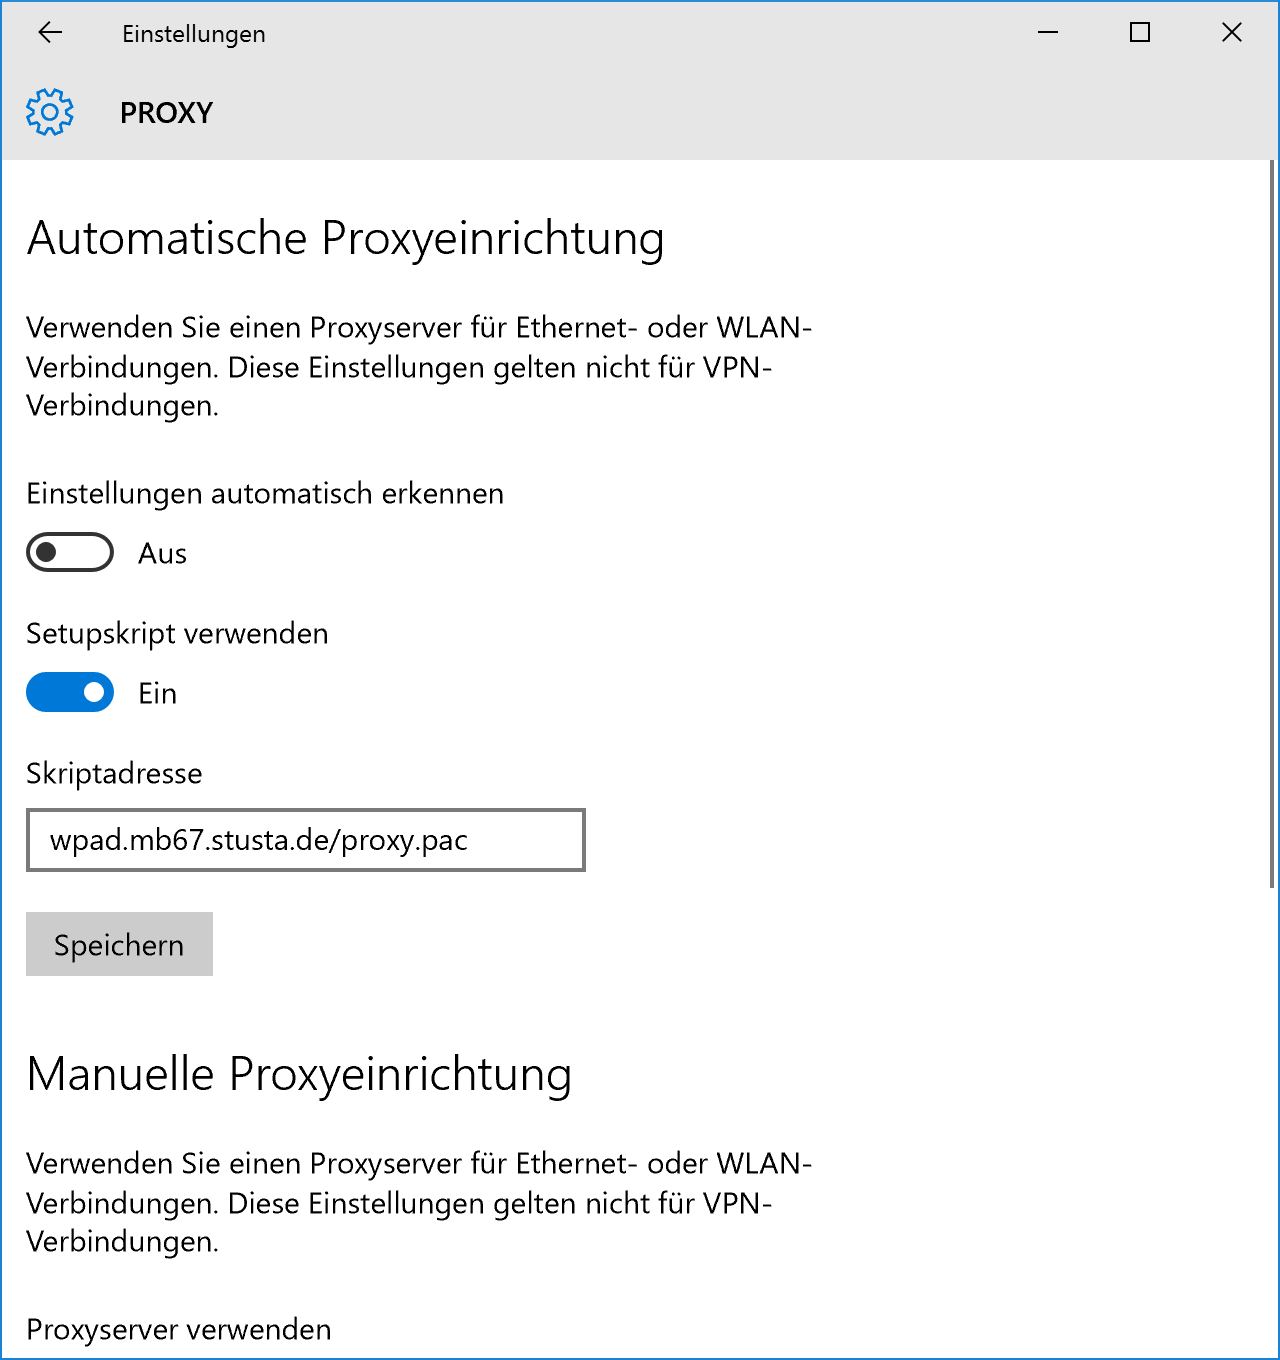
\includegraphics[width=0.4\textwidth,keepaspectratio]{Bilder/Proxy_Edge}
	\end{center}
	%  \vspace{-20pt}
	%	\caption{Eintragen des Proxyskripts in Microsoft Edge}
	%  \vspace{-10pt}
\end{wrapfigure}


Unter Windows haben Sie die Möglichkeit den Proxy global zu definieren.

\begin{enumerate}
	\item Suche \textit{Proxyeinstellungen ändern} in der Windows Suche eingeben und starten.
	\item Deaktivieren Sie die Option \emph{Einstellungen automatisch erkennen}.
	\item Wählen Sie \emph{Setupskript verwenden} und tragen Sie bei der Adresse \\ \url{http://wpad.stusta.mhn.de/proxy.pac} ein.
	\item Klicken Sie auf speichern und schließen Sie die geöffneten Fenster.
\end{enumerate}



\pagebreak

\begin{figure}[t!]
	\raggedleft
	\vspace{-20pt}
	
\includegraphics[height=1cm,keepaspectratio]{Bilder/linux_logo_neu}
	\vspace{-30pt}
\end{figure}



\subsubsection*{Anleitung fürs die globale Einstellung des Proxys unter Linux}

\paragraph*{} ~\\
\\
Unter Linux haben Sie die Möglichkeit den Proxy global zu definieren, sodass dieser nicht extra für jedes Programm eingetragen werden muss.
\begin{enumerate}
	\item Öffnen Sie die Netzwerk-Proxy-Einstellungen durch Klick auf \emph{System} $\rightarrow$ \emph{Einstellungen} $\rightarrow$ \emph{Netzwerk-Proxy}.
	\item Hier markieren Sie ganz unten die Option \emph{Automatische Proxy-Konfiguration} und tragen bei URL für Auto-Konfiguration: \url{http://wpad.stusta.mhn.de/proxy.pac} ein. Schließen Sie das Fenster. 
\end{enumerate}



\newpage
\enlargethispage{20pt}



\begin{figure}[t!]
	\raggedleft
	\vspace{-20pt}
	
\includegraphics[height=1cm,keepaspectratio]{Bilder/apple_logo_neu}
	\vspace{-30pt}
\end{figure}
\subsubsection*{Anleitung fürs die globale Einstellung des Proxys unter MacOS}

\\
Unter MacOS haben Sie die Möglichkeit den Proxy global zu definieren, sodass dieser nicht extra für jedes Programm eingetragen werden muss. Firefox benötigt allerdings trotzdem eine gesonderte Einstellungen (siehe Browsereinstellungen). %noch aktuelle info??

%\begin{wrapfigure}{r}{0.4\textwidth}
%  \vspace{-20pt}
%  \begin{center}
%    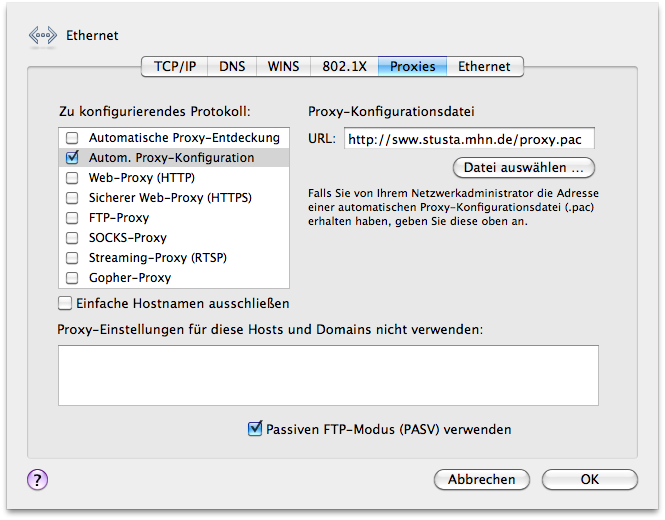
\includegraphics[width=0.48\textwidth,keepaspectratio]{Bilder/Proxy_MAC}
%  \end{center}
%  \vspace{-20pt}
%  \caption{Beispielhafte Proxyeinstellungen unter Mac OS~X}
%  \vspace{-10pt}
%\end{wrapfigure}
\begin{enumerate}%WTF 1. punkt???
    \item Öffnen Sie mit dem Button \emph{Weitere Optionen...} im voherigen Dialog die Detaileinstellungen und wechseln sie auf die Registerkarte \emph{Proxies}
    \item Setzen sie bei Zu konfigurierendes Protokoll vor Autom. Proxy-Konfiguration einen Hacken und tragen rechts bei URL \url{http://wpad.stusta.mhn.de/proxy.pac} ein. Schließen Sie die Detaileinstellungen mit OK und bestätigen Sie erneut mit Anwenden. Sie können die Netzwerkeinstellungen jetzt schließen.
\end{enumerate}

\newpage

\section*{Proxy-Konfiguration im Browser (nur Nicht-Mitglieder)}
\label{Proxy}

\begin{wrapfigure}{r}{0.5\textwidth}
	\vspace{-40pt}
	\begin{center}
		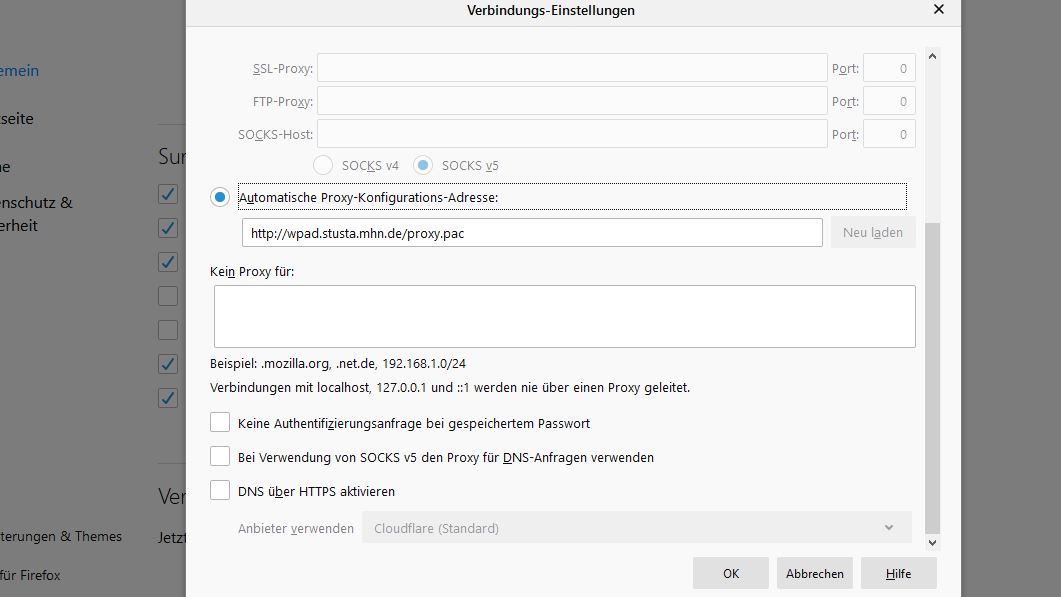
\includegraphics[width=0.5\textwidth,keepaspectratio]{Bilder/Firefox_neu_proxy}
	\end{center}
	%  \vspace{-20pt}
%	\caption{Eintragen des Proxyskripts in Mozilla Firefox}
	%  \vspace{-10pt}
\end{wrapfigure}

\subsection*{
\includegraphics[height=1.2cm,keepaspectratio]{Bilder/Firefox_35_logo} Mozilla Firefox}
\begin{enumerate}
	\item Klicken Sie auf die 3 übereinanderliegenden Striche in der rechten oberen Ecke, wählen Sie danach \emph{Einstellungen}.
	\item Gehen Sie zum Punkt \emph{Verbindungs-Einstellungen} und wählen diesen aus.
	\item Markieren Sie den Punkt \emph{Automatische Proxy-Konfigurations-Adresse} und tragen Sie als Automatische Proxy-Konfigurations-URL: \\ \url{http://wpad.stusta.mhn.de/proxy.pac} ein.
	\item Bestätigen Sie mit OK .\\
	\\
	\\
\end{enumerate}




\subsection*{
\includegraphics[height=1.2cm,keepaspectratio]{Bilder/Chrome_2011_logo} Google Chrome}
\begin{enumerate}
	\item Chrome starten.
	\item Klicken Sie auf die 3 übereinanderliegenden Striche in der rechten oberen Ecke, wählen Sie danach \emph{Einstellungen}.
	\item Wählen Sie den Punkt \emph{Erweiterte Einstellungen anzeigen}.
	\item Klicken Sie auf \emph{Proxy-Einstellungen des Computers öffnen}.
	\\
	\\
\end{enumerate}

%\newpage
%\begin{wrapfigure}{r}{0.5\textwidth}
%%  \vspace{-20pt}
%  \begin{center}
%    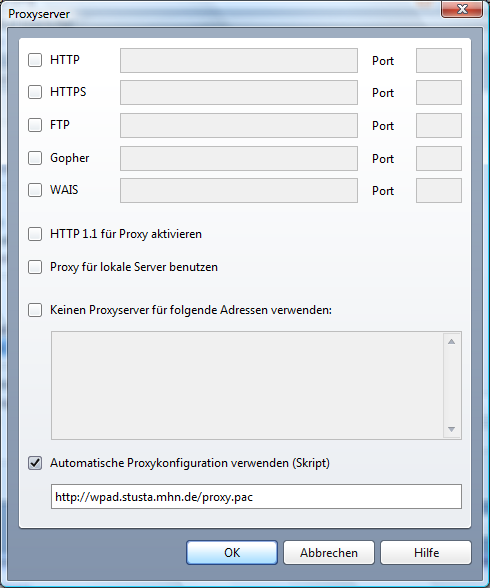
\includegraphics[width=0.5\textwidth,keepaspectratio]{Bilder/Proxy_Opera}
%  \end{center}
%%  \vspace{-20pt}
%  \caption{Eintragen des Proxyskripts im Opera}
%%  \vspace{-10pt}
%\end{wrapfigure}
%
%\subsection*{
\includegraphics[height=1.2cm,keepaspectratio]{Bilder/Opera_O} Opera}
%\begin{enumerate}
%    \item Opera starten.
%    \item Wählen Sie im Untermenü Extras den Punkt Einstellungen...
%    \item Wählen Sie im Reiter Erweitert auf der linken Seite die Kategorie Netzwerk und dann klicken Sie auf den Button Proxy.
%    \item Setzen Sie bei Automatische Proxykonfiguration verwenden (Skript) einen Haken und tragen Sie \\ \url{http://wpad.mb67.stusta.mhn.de/proxy.pac} ein.
%    \item Schließen Sie beide Fenster mit OK.
%\end{enumerate}
%$\rightarrow$ Der Internetzugang ist nun fertig konfiguriert.


\end{document}
